To subtract two numbers we use an subtraction process that mimics the behavior of arithmetic circuits for subtracting two bits binary numbers shown in 
\refFig{tra_subtract_circuit}.
\refFig{tra_subttraction} shows visualization of the subtraction process and the ABC code.
The full implementation of $Sub$ processes can be found in the appendix.
\begin{figure}[H]%
\centering
\fbox{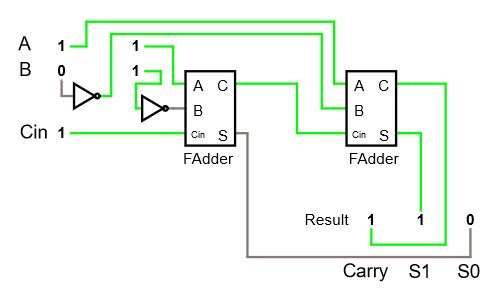
\includegraphics[keepaspectratio]{./images/transformational_semantics_of_oz/subtract_circuit.png}}
\caption{subtractor circuit}
\label{tra_subtract_circuit}%
\end{figure}
\begin{figure}[H]%
\centering
\subcaptionbox{ABC code.}{\fbox{$(\ \widehat{}\ \text{a,b,c}\ )\ (\ \text{Three}(\text{a})\ \mid\ \ \text{One}(\text{b})\ \mid\ \ \text{Sub}(\text{a,b,c})\ )$}}%
\hspace{\fill}
\subcaptionbox{Before subtraction.}{\fbox{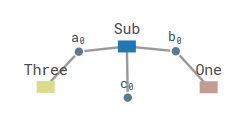
\includegraphics[keepaspectratio,width=0.45\textwidth]{./images/transformational_semantics_of_oz/sub_before.png}}}%
\hspace{1em}%
\subcaptionbox{After subtraction.}{\fbox{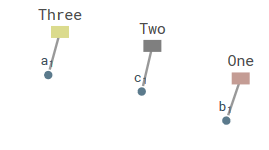
\includegraphics[keepaspectratio,width=0.45\textwidth]{./images/transformational_semantics_of_oz/sub_after.png}}}%
\caption{subtraction as a process}
\label{tra_subttraction}%
\end{figure}
